\documentclass[conference]{IEEEtran}
\usepackage{graphicx}
\usepackage{amsmath}
\usepackage{url}
\usepackage[hidelinks]{hyperref}

\begin{document}

\title{Reproducing Logic-LM: Symbolic Solvers for\\Faithful Logical Reasoning with LLMs}

\author{\IEEEauthorblockN{[FILL: Your Name] \quad Roll No.\ [FILL]}
\IEEEauthorblockA{[FILL: Department, College]\\
Code: \url{https://github.com/suriyakala-gif/Logic-LLM} (release v1.0.0)}}

\maketitle

\begin{abstract}
This report reproduces Table~2 of Logic-LM~\cite{pan2023logiclm}, in which
GPT-4 translates logical reasoning problems into symbolic programs that
deterministic solvers execute. Using the authors' released GPT-4 programs, I
re-ran the solver stage and evaluation on all five datasets with three seeds on
a free Colab CPU. Nine documented fixes were needed, including a Python~3.13
incompatibility that silently broke the constraint solver. Three datasets match
the paper within 0.2\%, while FOLIO and AR-LSAT are 8.3\% and 23.9\% lower. The
outcome is \textbf{Partly reproduced}: solver results match exactly, but the
chain-of-thought fallback answers were not released.
\end{abstract}

\begin{IEEEkeywords}
reproducibility, neuro-symbolic reasoning, large language models, symbolic solvers
\end{IEEEkeywords}

\section{Paper and Claim}
Pan et al.~\cite{pan2023logiclm} propose Logic-LM, which splits logical
reasoning into three stages: an LLM formulates the problem as a symbolic
program, a solver executes it (Pyke for ProntoQA and ProofWriter, Prover9 for
FOLIO, python-constraint for LogicalDeduction, Z3 for AR-LSAT), and the output
is mapped back to an answer. If a program cannot be executed, the method falls
back to a chain-of-thought (CoT) answer. The paper claims that this
outperforms standard and CoT prompting on all five benchmarks.

I reproduce the GPT-4 Logic-LM column of Table~2 (without self-refinement), and
compare executable rate (Exe\_Rate) and executable accuracy (Exe\_Acc) with
Table~3. The authors released the GPT-4 programs, so the solver stage can be
tested without paid API calls.

\section{Method}
\textbf{Setup.} Google Colab CPU runtime (2 vCPU, 12\,GB RAM, no GPU),
Ubuntu~24.04.5, Python~3.13.18, run on 9~Nov.~2026. I forked the original
repository (commit \texttt{d29f1e5}). The eight solver packages are pinned in
\texttt{requirements.txt}.

\textbf{Procedure.} For each dataset (dev split: 500, 600, 204, 299 and 230
problems) I ran the authors' \texttt{logic\_inference.py} and
\texttt{evaluation.py} on the saved programs, through a wrapper that sets
\texttt{random.seed}, with seeds 0, 1 and 2. Results are reported as mean
$\pm$ standard deviation. The whole run takes about 6~minutes.

\textbf{What I reduced.} No LLM calls were made, and self-refinement was not
run; both are consistent with Table~2. Non-executable programs use the
repository's \emph{random} backup, because the CoT answers used in the paper
are not released.

\textbf{Repository.} \url{https://github.com/suriyakala-gif/Logic-LLM}

\section{Results}
Table~\ref{tab:results} and Fig.~\ref{fig:results} compare my results with the
paper. ProntoQA and LogicalDeduction match exactly, and ProofWriter is within
0.2\%. FOLIO ($-8.3$\%) and AR-LSAT ($-23.9$\%) are lower. However, my
executable rate and the accuracy on executed programs match Table~3 on all
five datasets (e.g.\ FOLIO 80.37 vs.\ 80.4, AR-LSAT 60.00 vs.\ 60.0). The
gaps therefore come only from the 41 FOLIO and 155 AR-LSAT programs that do
not execute. The paper answers these with CoT; I could only guess randomly,
which also explains the larger seed variance on those two datasets.

\begin{table}[t]
\caption{Logic-LM (GPT-4) on the dev split: paper~\cite{pan2023logiclm}
vs.\ this reproduction (mean $\pm$ std, 3 seeds). Exe\_Rate and Exe\_Acc are
given as paper\,/\,mine.}
\label{tab:results}
\centering\footnotesize
\setlength{\tabcolsep}{2.5pt}
\begin{tabular}{lccrcc}
\hline
Dataset & Paper & Mine & Diff.\,(\%) & Exe\_Rate & Exe\_Acc \\
\hline
ProntoQA     & 83.20 & 83.20 $\pm$ 0.00 & $+0.0$  & 100.0\,/\,100.0 & 83.2\,/\,83.20 \\
ProofWriter  & 79.66 & 79.50 $\pm$ 0.17 & $-0.2$  & 99.0\,/\,99.0   & 79.6\,/\,79.63 \\
FOLIO        & 78.92 & 72.39 $\pm$ 2.83 & $-8.3$  & 79.9\,/\,79.6   & 80.4\,/\,80.37 \\
LogicalDed.  & 87.63 & 87.63 $\pm$ 0.00 & $+0.0$  & 100.0\,/\,100.0 & 87.6\,/\,87.63 \\
AR-LSAT      & 43.04 & 32.75 $\pm$ 2.66 & $-23.9$ & 32.6\,/\,32.6   & 60.0\,/\,60.00 \\
\hline
\end{tabular}
\end{table}

\begin{figure}[t]
  \centering
  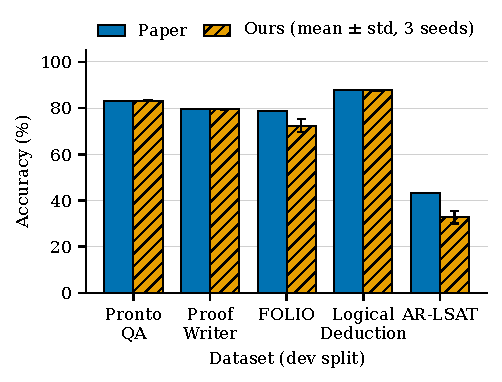
\includegraphics[width=\columnwidth]{fig1.pdf}
  \caption{Accuracy of Logic-LM with GPT-4 programs (no self-refinement) on the
  dev split of five logical reasoning benchmarks. Solid bars: values reported
  in~\cite{pan2023logiclm}. Hatched bars: this reproduction (mean $\pm$ std
  over 3 seeds of the random fallback). Three datasets match. FOLIO and
  AR-LSAT are lower only because failed programs fall back to random answers
  instead of the unreleased CoT answers.}
  \label{fig:results}
\end{figure}

\section{Problems and Fixes}
All attempts and logs are in \texttt{NOTES.md} and \texttt{logs/}.
\begin{enumerate}
  \item \textbf{Installation (attempts 1--5).} The authors'
  \texttt{requirements.txt} is a 139-line conda snapshot with local paths
  (\texttt{/croot/...}), so it fails immediately. Without those lines, the old
  pin \texttt{blis==0.7.10} does not build on Python~3.13. The Pyke package is
  actually named \texttt{scitools-pyke}, and it imports \texttt{imp}, a module
  removed in Python~3.12. I installed only the eight needed packages and
  restored \texttt{imp} with \texttt{zombie-imp}.
  \item \textbf{Missing dependency (6).} The FOLIO parser needs \texttt{ply},
  which is not listed anywhere.
  \item \textbf{Out of memory (7).} FOLIO was killed at problem 68/204 (exit
  code 137): one program exhausts the 12\,GB RAM. A 4\,GB cap
  (\texttt{ulimit -v}) makes it fail cleanly and fall back.
  \item \textbf{Python~3.13 bug (8--9).} LogicalDeduction executed 0/299
  programs and then crashed, because \texttt{random\_backup()} does not support
  this dataset. Debugging showed that the CSP programs were valid, but
  \texttt{exec()} followed by \texttt{locals()} loses the answer under
  Python~3.13 (PEP~667). A two-line change to execute into an explicit
  dictionary restored 299/299 executions and 87.63\% accuracy.
\end{enumerate}
\textbf{Missing from the paper or repository:} the Python version, a usable
dependency list, the CoT answers used as the fallback, and memory or time
limits. The README's output folder name also differs from the code's. The
FOLIO Exe\_Rate varied between runs (78.92\% or 79.90\%), because one program
sits at the solver timeout. \textbf{Code changed:} only the two lines in
\texttt{csp\_solver.py}.

\section{Assessment}
The paper is \emph{reproducible at the solver level}. With the released
programs, all five executable rates and executable accuracies match Table~3,
and three of the five accuracies in Table~2 match exactly. It is \emph{not
fully reproducible end-to-end}: the CoT fallback answers are not released, the
programs come from a closed and changing API model, and the environment is not
specified, so a current Python silently produces wrong results without any
error message.

\textbf{Extension.} The programs could be regenerated with an open-weight model
(e.g.\ Llama or Qwen) and a released, versioned CoT fallback. That would make
the whole pipeline reproducible offline and would show how much of Logic-LM's
gain depends on GPT-4's translation quality.

\bibliographystyle{IEEEtran}
\bibliography{refs}

\vspace{4pt}
\noindent\textit{AI tools were used to help debug code and structure this
report; all reported numbers come from my own runs.}

\end{document}
